\clearpage
\begin{explanationbox}

\textbf{\textcolor{CExplanation}{为什么会想到研究这些性质？}}

遇到 $2^x$、$(1/2)^x$，如果每次比较大小都先算出小数，既慢又容易出错。我们更想知道：\textbf{只看底数，能否判断图像往哪边走、经过哪里、什么时候大于 $1$？} 这就是整理指数函数性质的目的。

\medskip
\textbf{\textcolor{CExplanation}{快懂一：把指数看成“连续乘多少次”}}
\begin{center}\begin{tikzpicture}[font=\small,>=stealth,line join=round]
\draw[gray!40,rounded corners=3pt] (0,0) rectangle (14.2,8.8);\node at (7.1,8.200000000000001) {看见每次乘底数：横着走同样一步，高度按倍数改变};
\node at (3.1500000000000004,7.3) {$y=2^x$};\begin{scope}[shift={(1.3758620689655174,3.3000000000000003)},x=1.6896551724137934cm,y=0.6cm]\draw[->,gray] (-0.4,0)--(2.5,0) node[right]{$x$};\draw[->,gray] (0,-0.5)--(0,5) node[above]{$y$};\draw[blue!75!black,thick,solid,domain=-0.2:2.2,samples=180] plot(\x,{pow(2,\x)});\fill[orange!85!black] (0,1) circle(2pt);\fill[orange!85!black] (1,2) circle(2pt);\fill[orange!85!black] (2,4) circle(2pt);\node[below left=5pt] at (0,0){$0$};\node[below=5pt] at (1,0){$1$};\node[below=5pt] at (2,0){$2$};\draw[gray,densely dotted] (1,0)--(1,2);\draw[gray,densely dotted] (2,0)--(2,4);\draw[->,blue!75!black,thick] (.2,1.148698354997035)--(.8,1.7411011265922482);\draw[->,blue!75!black,thick] (1.2,2.2973967099940698)--(1.8,3.4822022531844965);\end{scope}\node[align=center,text width=5.8cm] at (3.1500000000000004,1.7) {$x:0\to1\to2$\\$y:1\to2\to4$，每步乘$2$};\node at (9.95,7.3) {$y=(\frac12)^x$};\begin{scope}[shift={(8.175862068965518,3.3000000000000003)},x=1.6896551724137934cm,y=0.6cm]\draw[->,gray] (-0.4,0)--(2.5,0) node[right]{$x$};\draw[->,gray] (0,-0.5)--(0,5) node[above]{$y$};\draw[orange!80!black,thick,solid,domain=-0.2:2.2,samples=180] plot(\x,{pow(0.5,\x)});\fill[orange!85!black] (0,1.0) circle(2pt);\fill[orange!85!black] (1,0.5) circle(2pt);\fill[orange!85!black] (2,0.25) circle(2pt);\node[below left=5pt] at (0,0){$0$};\node[below=5pt] at (1,0){$1$};\node[below=5pt] at (2,0){$2$};\draw[gray,densely dotted] (1,0)--(1,0.5);\draw[gray,densely dotted] (2,0)--(2,0.25);\draw[->,orange!80!black,thick] (.2,0.8705505632961241)--(.8,0.5743491774985174);\draw[->,orange!80!black,thick] (1.2,0.43527528164806206)--(1.8,0.2871745887492587);\end{scope}\node[align=center,text width=5.8cm] at (9.95,1.7) {$x:0\to1\to2$\\$y:1\to\frac12\to\frac14$，每步减半};
\node[text width=12.6cm,align=center] at (7.1,.65) {两图同尺度；整数点帮助理解作图，任意实数的证明还要看后面的倍数法。};
\end{tikzpicture}\end{center}

\textbf{观察：}横坐标每次增加1，点的高度按倍数变化。\quad\textbf{原因：}a的x+1次方等于a乘a的x次方。

\textbf{考试使用：}先画三个关键点，再连光滑曲线；整数表不代替实数证明。



例如，一份学习资料的数量每天变成前一天的 $2$ 倍。从开始那天记作第 $0$ 天，数量按 $2^x$ 变化；如果每天只剩前一天的一半，则按 $(1/2)^x$ 变化。$x=-1,-2$ 可以理解为往前倒推一两步。
\[
\begin{array}{c|ccccc}
    x & -2&-1&0&1&2\\\hline
    2^x & \frac14&\frac12&1&2&4\\
    (\frac12)^x &4&2&1&\frac12&\frac14
\end{array}
\]
\textbf{从表里看出三件事：}两行在 $x=0$ 都是 $1$；一行从左到右越来越大，另一行越来越小；两行的数值以 $x=0$ 为中心左右对换。

\end{explanationbox}
\clearpage
\begin{explanationbox}
\begin{center}
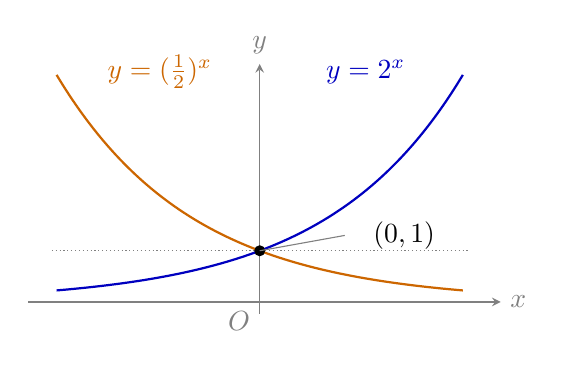
\begin{tikzpicture}[x=1.2cm,y=0.65cm,>=stealth]
  \draw[->,gray] (-2.45,0) -- (2.55,0) node[right] {$x$};
  \draw[->,gray] (0,-0.23) -- (0,4.65) node[above] {$y$};
  \draw[densely dotted,gray] (-2.2,1) -- (2.2,1);
  \draw[blue!75!black,thick,smooth] plot[domain=-2.15:2.15,samples=70] (\x,{pow(2,\x)});
  \draw[orange!80!black,thick,smooth] plot[domain=-2.15:2.15,samples=70] (\x,{pow(2,-\x)});
  \fill (0,1) circle (2pt);
  \draw[gray] (0,1)--(.9,1.3);\node[anchor=west] at (1.1,1.3) {$(0,1)$};
  \node[blue!75!black,anchor=west] at (.6,4.5) {$y=2^x$};
  \node[orange!80!black,anchor=east] at (-.4,4.5) {$y=(\frac12)^x$};
  \node[gray,anchor=north east] at (0,0) {$O$};
\end{tikzpicture}
\end{center}
\textbf{画图方法：}分别标出 $(-1,\frac12),(0,1),(1,2)$ 与 $(-1,2),(0,1),(1,\frac12)$，再顺着增减方向连成光滑曲线。图是为了看懂方向，不能代替严谨证明。

\medskip

\end{explanationbox}
\clearpage
\begin{explanationbox}
\textbf{\textcolor{CExplanation}{快懂二：为什么恰好在 $(0,1)$ 相遇？}}
\begin{center}\begin{tikzpicture}[font=\small,>=stealth,line join=round]
\draw[gray!40,rounded corners=3pt] (0,0) rectangle (14.2,8.3);\node at (7.1,7.700000000000001) {底数从4减到1/4：右侧降低，左侧升高，仍过(0,1)};
\begin{scope}[shift={(4.1,2.0951612903225807)},x=1.1538461538461537cm,y=0.7419354838709677cm]\draw[->,gray] (-2.6,0)--(2.6,0) node[right]{$x$};\draw[->,gray] (0,-0.6)--(0,5.6) node[above]{$y$};\draw[violet,thick,solid,domain=-2.3:1.131517202916897,samples=180] plot(\x,{pow(4,\x)});\draw[blue!75!black,thick,dashed,domain=-2.3:2.263034405833794,samples=180] plot(\x,{pow(2,\x)});\draw[orange!80!black,thick,densely dotted,domain=-2.263034405833794:2.3,samples=180] plot(\x,{pow(0.5,\x)});\draw[teal,thick,dashdotted,domain=-1.131517202916897:2.3,samples=180] plot(\x,{pow(0.25,\x)});\fill[orange!85!black] (0,1) circle(2.2pt);\draw[gray,densely dotted] (-2.3,1)--(2.3,1);\node[below=5pt] at (-2,0){$-2$};\node[below left=5pt] at (0,0){$0$};\node[below=5pt] at (2,0){$2$};\end{scope}\node[anchor=west,align=left,text width=5.0cm] at (8.4,4.0) {底数依次减小：\\[5pt]紫$4$、蓝$2$、橙$\frac12$、青$\frac14$\\[9pt]固定$x>0$：高度降低\\[9pt]固定$x<0$：高度升高\\[9pt]$x=0$：高度始终为$1$};
\node[text width=12.6cm,align=center] at (7.1,.65) {“顺时针”描述共同点附近的走势；曲线会改变弯曲程度，并非整条刚性旋转。};
\end{tikzpicture}\end{center}

\textbf{观察：}固定左右各一个横坐标，分别看高度。\quad\textbf{原因：}x>0时正幂保序；x<0时先取倒数，大小反向。

\textbf{考试使用：}同一侧比较曲线高低，判断底数大小；不能跨左右照搬。



因为任何正底数都有 $a^0=1$，所以不管选 $2$、$3$ 还是 $\frac12$，把 $x=0$ 代进去都得到 $y=1$。反过来，$x=1$ 时得到 $y=a$，随底数而变，故 $(1,a)$ 不是所有指数函数共同经过的\textbf{定点}。

\medskip

\end{explanationbox}
\clearpage
\begin{explanationbox}
\textbf{\textcolor{CExplanation}{快懂三：为什么始终大于 $0$，却又能无限接近 $0$？}}
\begin{center}\begin{tikzpicture}[font=\small,>=stealth,line join=round]
\draw[gray!40,rounded corners=3pt] (0,0) rectangle (14.2,8.3);\node at (7.1,7.700000000000001) {越往右越接近0，但每个点仍有正的高度};
\begin{scope}[shift={(1.6660377358490566,2.191176470588235)},x=1.1320754716981132cm,y=3.3823529411764706cm]\draw[->,gray] (-0.5,0)--(4.8,0) node[right]{$x$};\draw[->,gray] (0,-0.16)--(0,1.2) node[above]{$y$};\draw[orange!80!black,thick,dashed,domain=0:4.3,samples=180] plot(\x,{pow(2,-\x)});\fill[orange!85!black] (1,0.5) circle(2.2pt);\fill[orange!85!black] (3,0.125) circle(2.2pt);\fill[orange!85!black] (4,0.0625) circle(2.2pt);\node[below left=5pt] at (0,0){$0$};\node[below=5pt] at (1,0){$1$};\node[below=5pt] at (3,0){$3$};\node[below=5pt] at (4,0){$4$};\node[left=5pt] at (0,1){$1$};\draw[orange!80!black,densely dotted] (1,0)--(1,0.5);\draw[orange!80!black,densely dotted] (3,0)--(3,0.125);\draw[orange!80!black,densely dotted] (4,0)--(4,0.0625);\end{scope}\node[anchor=west,align=left,text width=5.0cm] at (8.4,4.0) {$y=(\frac12)^x$\\[9pt]$x=1:\ y=\frac12$\\[9pt]$x=3:\ y=\frac18$\\[9pt]$x=4:\ y=\frac1{16}>0$\\[9pt]值域$(0,+\infty)$，不含$0$};
\node[text width=12.6cm,align=center] at (7.1,.65) {每多乘一次二分之一，高度更小却仍为正；画在横轴附近，不表示落到了横轴上。};
\end{tikzpicture}\end{center}

\textbf{观察：}小高度仍在横轴上方。\quad\textbf{原因：}每次除以2，正数仍是正数。

\textbf{考试使用：}值域端点0用圆括号，不写最小值为0。



先想 $2^{-1}=\frac12,\ 2^{-2}=\frac14,\ 2^{-3}=\frac18$。往左走，分母不断变大，值越来越靠近 $0$，但每一项仍是正数。对于任何 $a>0$，$a^x$ 都是正数；把底数换成 $\frac12$，靠近 $0$ 的方向改成向右。因此 $y=0$ 是图像靠近但永远碰不到的水平直线；另一侧的函数值能不断增大，所以\textbf{全部可能的函数值恰好是正数}。

\medskip

\end{explanationbox}
\clearpage
\begin{explanationbox}
\textbf{\textcolor{CExplanation}{快懂四：底数互为倒数，为什么图像左右翻转？}}
\begin{center}\begin{tikzpicture}[font=\small,>=stealth,line join=round]
\draw[gray!40,rounded corners=3pt] (0,0) rectangle (14.2,8.3);\node at (7.1,7.700000000000001) {关于y轴对称：横坐标变号，高度和距离都不变};
\begin{scope}[shift={(4.1,2.161111111111111)},x=1.0714285714285714cm,y=0.7301587301587301cm]\draw[->,gray] (-2.8,0)--(2.8,0) node[right]{$x$};\draw[->,gray] (0,-0.7)--(0,5.6) node[above]{$y$};\draw[blue!75!black,thick,solid,domain=-2.3:2.15,samples=180] plot(\x,{pow(2,\x)});\draw[orange!80!black,thick,dashed,domain=-2.3:2.15,samples=180] plot(\x,{pow(2,-\x)});\fill[orange!85!black] (-2,4) circle(2.2pt);\fill[orange!85!black] (2,4) circle(2.2pt);\fill[orange!85!black] (0,1) circle(2.2pt);\node[above=7pt] at (-1.25,4.65){$(-2,4)$};\node[above=7pt] at (1.25,4.65){$(2,4)$};\draw[<->,gray] (-2,4)--(0,4);\draw[<->,gray] (0,4)--(2,4);\node[below=4pt] at (-1,4){$2$};\node[below=4pt] at (1,4){$2$};\node[below=5pt] at (-2,0){$-2$};\node[below left=5pt] at (0,0){$0$};\node[below=5pt] at (2,0){$2$};\end{scope}\node[anchor=west,align=left,text width=5.0cm] at (8.4,4.0) {蓝：$f(x)=2^x$\\[8pt]橙：$g(x)=2^{-x}=f(-x)$\\[8pt]$(2,4)\leftrightarrow(-2,4)$\\[8pt]一般为$(t,f(t))$\\[4pt]$\leftrightarrow(-t,f(t))$};
\node[text width=12.6cm,align=center] at (7.1,.65) {同一水平线上的两点距y轴相等；从一条曲线可直接翻出另一条。};
\end{tikzpicture}\end{center}

\textbf{观察：}同一水平线的两点左右等距。\quad\textbf{原因：}倒数底数等于指数变号。

\textbf{考试使用：}对应点只改横坐标符号，交点为(0,1)。



\[
\left(\frac1a\right)^x=a^{-x}=f(-x).
\]
计算 $g(x)$ 等同于先把 $x$ 换成 $-x$，再交给 $f$。例如 $f(-2)=\frac14$，而 $g(2)=\frac14$；于是 $(-2,\frac14)$ 和 $(2,\frac14)$ 分居 $y$ 轴两侧、离它同样远。这就是\textbf{关于 $y$ 轴对称}，不是关于 $x$ 轴对称。

\medskip
\end{explanationbox}
\clearpage
\begin{explanationbox}

\begin{center}\begin{tikzpicture}[font=\small,>=stealth,line join=round]
\draw[gray!40,rounded corners=3pt] (0,0) rectangle (14.2,8.3);\node at (7.1,7.700000000000001) {为什么可以说顺时针？准确地看共同点处的切线};
\begin{scope}[shift={(4,3.9)},x=1.25cm,y=1.25cm]\draw[->,gray] (-2.2,0)--(2.2,0) node[right]{$x$};\draw[->,gray] (0,-1.3)--(0,2.4) node[above]{$y$};\draw[violet,thick,solid] (-.8,-0.10903548889591241)--(.8,2.1090354888959126);\draw[blue!75!black,thick,dashed] (-.8,0.4454822555520438)--(.8,1.5545177444479563);\draw[orange!80!black,thick,densely dotted] (-.8,1.5545177444479563)--(.8,0.4454822555520438);\draw[teal,thick,dashdotted] (-.8,2.1090354888959126)--(.8,-0.10903548889591241);\fill[orange!80!black] (0,1) circle(2pt);\draw[->,black] (1.15,2.15) arc[start angle=45,end angle=-45,radius=1.62635];\end{scope}\node[anchor=west,align=left,text width=5.1cm] at (8.2,4.2) {共同点$(0,1)$处的切线\\[8pt]底数$4\to2\to\frac12\to\frac14$\\[8pt]方向顺时针改变\\[8pt]高中导数核对：\\[5pt]$f\,\!\prime(0)=\ln a$};
\node[text width=12.6cm,align=center] at (7.1,.65) {底数减小，切线斜率随之减小；a=1时为水平线y=1，通常单列为常数函数。};
\end{tikzpicture}\end{center}

\textbf{观察：}只比较共同点处的短切线方向。\quad\textbf{原因：}高中可由导数验证切线斜率为ln a，随a减小而减小。

\textbf{考试使用：}顺时针是记忆方向，不能把整条曲线当直线旋转。

\end{explanationbox}
\clearpage
\begin{explanationbox}

\begin{center}\begin{tikzpicture}[font=\small,>=stealth,line join=round]
\draw[gray!40,rounded corners=3pt] (0,0) rectangle (14.2,8.8);\node at (7.1,8.200000000000001) {字母位置换了，变化的对象就不同};
\node at (3.1500000000000004,7.3) {$y=2^x$};\begin{scope}[shift={(2.7511627906976743,3.3535714285714286)},x=1.1395348837209303cm,y=0.5892857142857143cm]\draw[->,gray] (-1.8,0)--(2.5,0) node[right]{$x$};\draw[->,gray] (0,-0.6)--(0,5) node[above]{$y$};\draw[blue!75!black,thick,solid,domain=-1.5:2.2,samples=180] plot(\x,{pow(2,\x)});\fill[orange!85!black] (0,1) circle(2pt);\node[below left=5pt] at (0,0){$0$};\node[below=5pt] at (1,0){$1$};\end{scope}\node[align=center,text width=5.8cm] at (3.1500000000000004,1.7) {底数2固定\\指数x变化};\node at (9.95,7.3) {$y=x^2$};\begin{scope}[shift={(9.551162790697674,3.3535714285714286)},x=1.1395348837209303cm,y=0.5892857142857143cm]\draw[->,gray] (-1.8,0)--(2.5,0) node[right]{$x$};\draw[->,gray] (0,-0.6)--(0,5) node[above]{$y$};\draw[teal,thick,solid,domain=-1.5:2.2,samples=180] plot(\x,{\x*\x});\fill[orange!85!black] (0,0) circle(2pt);\node[below left=5pt] at (0,0){$0$};\node[below=5pt] at (1,0){$1$};\end{scope}\node[align=center,text width=5.8cm] at (9.95,1.7) {指数2固定\\底数x变化};
\node[text width=12.6cm,align=center] at (7.1,.65) {两图同尺度；指数函数过(0,1)，平方函数过原点，负半轴走势也不同。};
\end{tikzpicture}\end{center}

\textbf{观察：}同样的2和x，图像过点与负半轴走势不同。\quad\textbf{原因：}一个固定底数，一个固定指数。

\textbf{考试使用：}先看字母在哪个位置，再使用相应性质。

\textbf{\textcolor{CExplanation}{连接旧知识与考试使用}}
\begin{itemize}[leftmargin=*,itemsep=0.4em,topsep=0.3em]
  \item \textbf{连接负指数：}$a^{-n}=1/a^n$，这同时解释了左侧数值和图像的左右翻转。
  \item \textbf{连接单调性：}同底比较先看底数，$a>1$ 时指数大者值大；$0<a<1$ 时恰好相反。
  \item \textbf{连接幂函数：}$a^x$ 是\textbf{底数固定、指数变化}；$x^a$ 是\textbf{底数变化、指数固定}，名字容易混淆，规律不能照搬。
\end{itemize}

\textbf{\textcolor{CExplanation}{顿悟点：}}\textbf{“$x$ 每加 $1$，值乘 $a$”是增减性的起点；“$a^0=1$”是定点的起点；“倒数等于指数变号”是对称性的起点。}

\end{explanationbox}
